
\chapter{Characterizing Chemotactic Performance}


\section{Survey of Chemotactic Index}

The most common way of measuring the performance of cell chemotaxis is by calculating the chemotactic index (CI) from cell motility experiments. The CI is supposed to give quantitative measure of chemotaxis performance, however how CI is calculated from experiments often varies from study to study. CI has been defined as the ratio of the distance traveled towards the chemoattractant to the distance traveled in the absence of chemoattractant \cite{nelson1975chemotaxis}, the ratio of the number of cells that migrate in response to chemokine to the number of cells that migrate in the absence of stimulus \cite{iellem2001unique,mayr2002vascular,fiedler2005vegf}, and the cosine of the angle made by the cell's displacement vector and the gradient direction
\cite{mouneimne2006spatial,kay2008changing,funamoto2001role}.

\begin{figure}
    \centering
        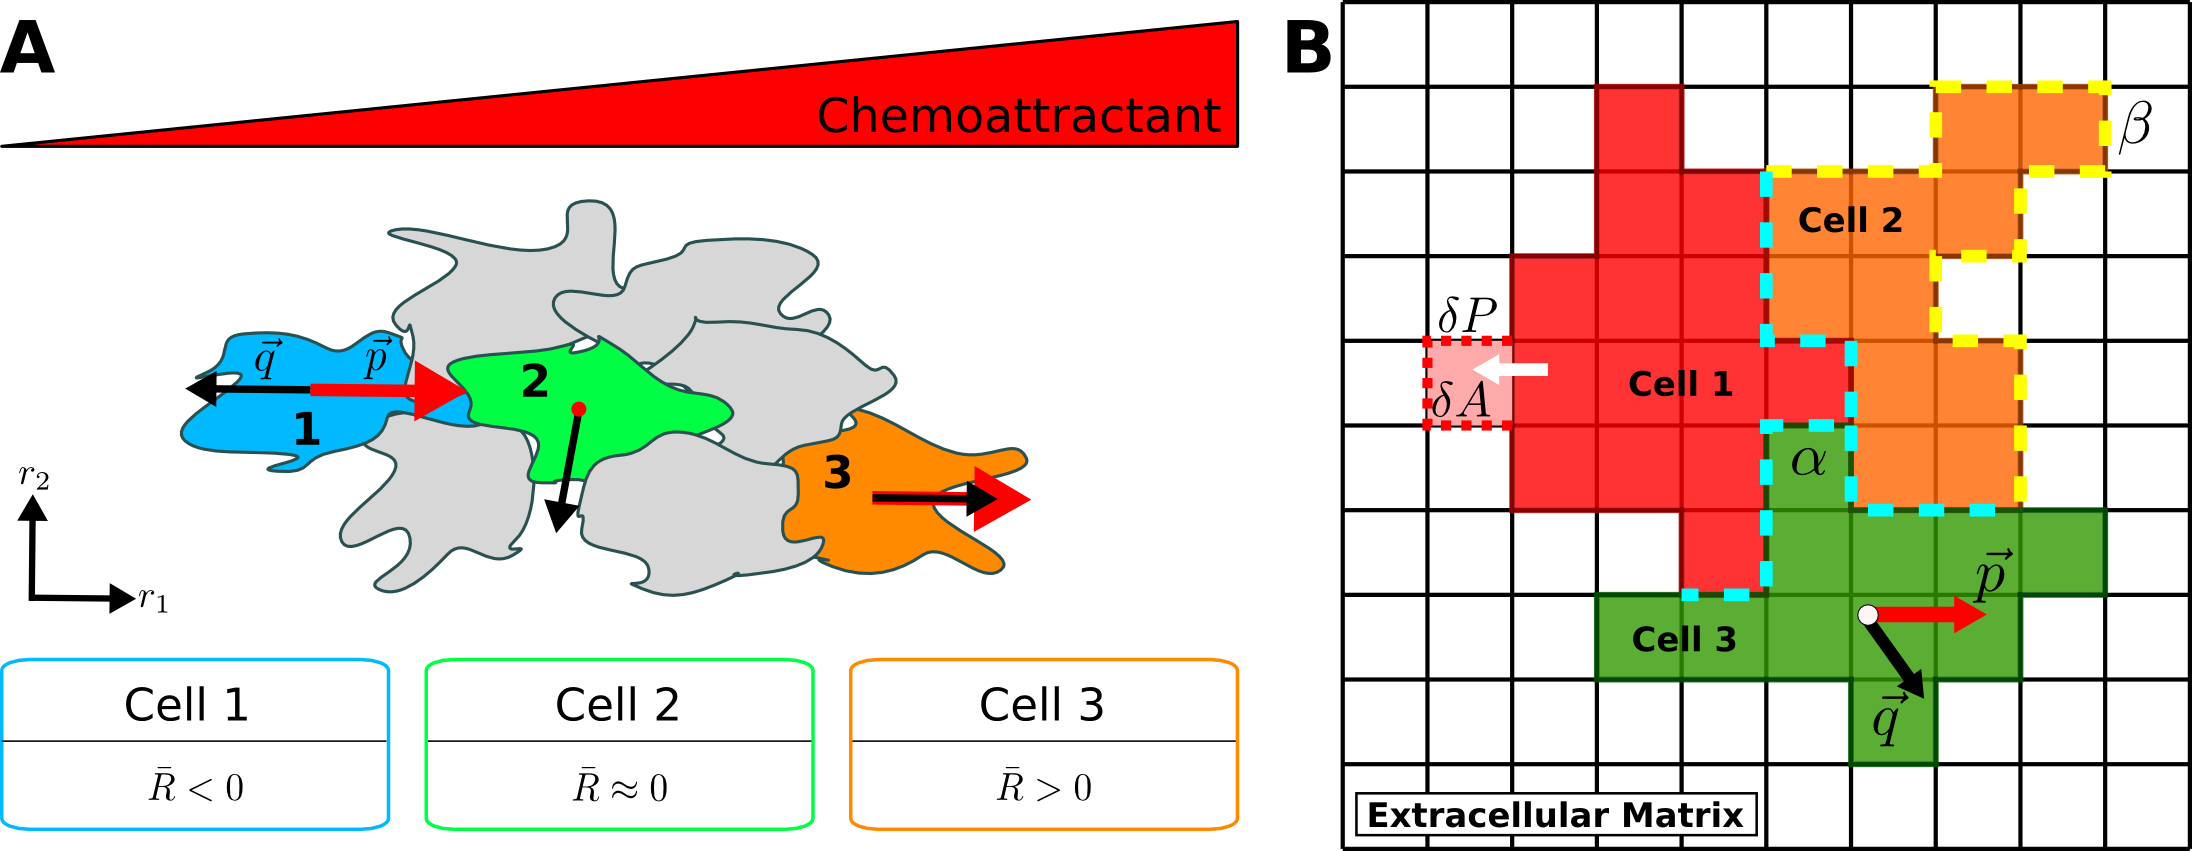
\includegraphics[width=.40\textwidth]{../fig/ch4_fig1.png}
    \caption{Illustration of chemotaxis. The cell or cluster's trajectory is traced out in grey. $\theta$ is the angle made between the direction of the gradient and the net displacement of cell or cluster.} \label{fig:ch4_f1}
\end{figure}

The latter two definitions are very commonly found in the literature although comparing them between different experiments is unclear. The definition based on the ratio of numbers of cells gives a measure of the increase in migratory response when cells are in exposed to a certain chemokine. With this definition $\text{CI} = 1$ corresponds to no chemotactic response and $\text{CI} > 1$ represents increased response. The definition based on the angle of a single cell's migration measures how accurate cells are in identifying the gradient direction, and is defined as the average of $\cos\theta$ over many cell trajectories:
\begin{equation}
    \text{CI} = \langle \cos\theta \rangle \ .
\end{equation}
In this case $\text{CI} = 1$ represents perfectly accurate chemotaxis, with the cell's displacement pointing parallel to the gradient direction.

\section{Chemotactic Ratio}

A final method of quantifying chemotaxis is with the Chemotactic Ratio (CR) McCutcheon index, which is defined as the ratio of the total displacement of the cell from moving from its start to end point to the net distance traveled.
\begin{equation}
    \text{CR} = \frac{\text{displacement}}{\text{distance}}
\end{equation}
In this case $\text{CR} = 1$ represents perfectly efficient chemotaxis, the cell did travel more than the minimal distance to get from its start-point to its endpoint. The chemotactic ratio is also known as the McCutcheon Index \cite{mccutcheon1946chemotaxis} and the straightness index \cite{codling2008random}.

The measures $\text{CI} = \cos\theta$ and $\text{MI} = \frac{\text{displacement}}{\text{distance}}$ are both very useful metrics for characterizing chemotaxis performance. The closer to $1$ CI is to more accurate the cells are, whereas a CI value $\approx 0$ indicates that there is very little to no chemotactic response and the cells' motion is in general unbiased. MI on the other hand quantifies the efficiency with which cells migrate during chemotaxis. A small MI value indicates inefficient chemotaxis since the cells are traveling a large distance for very little net displacement.

Can we relate these two metric of chemotactic performance to the fundamental limits of cell gradient sensing in order to understand chemotaxis' dependence on the mechanisms of gradient sensing and migration?


\section{Chemotactic Index \& Migration Performance}

How can does the chemotactic index quantify migratory performance? We can relate the statistics of migration to the chemotactic index by approximating the cell of cluster's motion as that of a random walk.

The simplest model is that of a one dimensional biased random walk. We assume that the walker is biased by a constant drift velocity $v$. The typical net displacement and total distance traveled by the walker will be due to both diffusion and drift:
\begin{gather}
    \Delta x_\text{net} = \sigma + \langle x \rangle \\
    \Delta x_\text{tot} = \frac{\sigma^2}{a} + \langle x \rangle ,
\end{gather}
with $a$ being the length of one step. The ratio of the displacement $\Delta x_\text{net}$ to the distance $\Delta x_\text{tot}$ is the chemotactic index measure MI. For a 1D biased random walk $\sigma = \sqrt{2Dt}$ with $D$ being the diffusion coefficient and $\langle x \rangle = vt$. In the long time limit this simplifies to
\begin{equation}
    \lim_{t\to\infty} \text{MI} = \frac{\eta}{2+\eta} ,
\end{equation}
with $\eta$ the Peclet number.

\begin{figure}
    \centering
        \includegraphics[width=.40\textwidth]{../fig/1dRW_drift_1.png}
    \caption{One dimensional biased random walk with drift velocity $\bar{v}$. The grey line indicates the distance travelled along the path taken by the walker, and the red line is the net displacement of the walker from its initial position.} \label{fig:rw}
\end{figure}

A more accurate description of the chemotaxis however should take into account that the bias in the random walk fluctuates. The bias $v$ is a random variable with mean $\bar{v}$ and variance $\sigma_v$. Therefore, the expressions for the biased random walker's displacement and distance become
\begin{gather}
    \Delta x_\text{net} = \sigma_v t + \bar{v}t \\
    \Delta x_\text{tot} = \frac{\sigma^2_v t^2}{a} + \bar{v} t.
\end{gather}
The chemotactic index can be written in terms of the migratory velocity's \textit{relative error}
$\epsilon^2 \equiv \sigma_v^2 / \bar{v}^2$,
and the dimensionless parameter
$\alpha \equiv a / \bar{v} t$,
\begin{equation}
    \text{MI}_{1\text{D}} = \frac{\epsilon + 1}{\epsilon^2\alpha^{-1}+1} .
\end{equation}
This formalism is not limited to random walks in one dimension but can be generalized to two and three dimensions by assuming that drift only occurs in one dimension (e.g.
$\bar{v}_x>0$, $\bar{v}_{y,z}=0$).
For cells of clusters that are free to move in three dimensions the chemotactic index becomes
\begin{equation} \label{eq:mi3d}
    \text{MI}_{3\text{D}} = \frac{\sqrt{(1+\epsilon)^2 + 2\epsilon^2}}
                            {3\epsilon^2\alpha^{-1}+1} .
\end{equation}

The other chemotactic index can be derived calculating the expecation value of $\cos \theta$. Assuming the the angle $\theta$ is a random variable sampled from a normal distribution,
$\theta \sim \mathcal{N}(\bar{\theta},\sigma_\theta^2)$, then
\begin{equation}
    \text{CI} = \langle \cos\theta \rangle = \int_{-\pi}^{\pi} d\theta \ \cos\theta \ \mathcal{N}(\bar{\theta},\sigma_\theta^2) .
\end{equation}
The angle $\theta$ depends on the cell of cluster's velocity in the directions parallel and perpendicular to the gradient,
$\theta \approx v_\perp / v_\parallel$. Assuming that $\bar{v}_\perp = 0$ and $\bar{v}_\parallel > 0$ the mean and variance of $\theta$ are (see SI)
\begin{gather}
    \bar{\theta} = \bar{v}_\perp / \bar{v}_\parallel = 0 \\
    \sigma_\theta^2 = 4\sigma_v^2 / \bar{v}^2_\parallel = 4 \epsilon^2 ,
\end{gather}
and the chemotactic index simplifies to
\begin{equation} \label{eq:ci3}
    \langle \cos\theta \rangle =
    % \frac{e^{-2\epsilon^2}}{2 \erf\left( \frac{\pi}{2\sqrt{2}\epsilon}\right)}
    % \left[ \erf\left( \frac{\pi-4i\epsilon^2}{2\sqrt{2}\epsilon} \right) + \erf\left( \frac{\pi+4i\epsilon^2}{2\sqrt{2}\epsilon} \right) \right]
    e^{-2\epsilon^2} \frac{
    \left[ \erf\left( \frac{\pi-4i\epsilon^2}{2\sqrt{2}\epsilon} \right) + \erf\left( \frac{\pi+4i\epsilon^2}{2\sqrt{2}\epsilon} \right) \right] }
    {2 \erf\left( \frac{\pi}{2\sqrt{2}\epsilon}\right)} .
\end{equation}
Interestingly, both chemotactic index metrics MI and $\langle \cos\theta \rangle$ are monotonically decreasing functions of the relative error as demonstrated by Eq.\ \ref{eq:mi3d} and Eq.\ \ref{eq:ci3}. Therefore these two measurements of CI measure the precision of chemotaxis. A value of CI close to 1 indicates very precise chemotaxis whereas CI close to 0 means that chemotaxis is imprecise.

This brings us back to our original motivating questions: what is the relative error in collective chemotaxis, and what are there ways to distinguish between different mechanisms of chemotaxis? Since the experimentally determined CI depends on the relative error $\epsilon^2$ understanding the functional form of $\epsilon^2$ may allow chemotactaxis experiments to categorize the migratory mechanisms in use. Here we focus on two broad categories of collective chemotaxis; one due to single-cell gradient sensing and the other arising from collective sensing. In the individual-based model cells make independently measure the chemoattractant and polarize themselves. In the collective model gradient sensing is done by sampling the chemoattractant across the whole cluster and cells on the exterior of the cluster polarize themselves accordingly. Below we describe the models in detail and then examine the expressions for the relative error in migratory velocity that arise from either mechanisms.
